\documentclass[11pt]{article}
\usepackage[margin=0.72in]{geometry}
\usepackage{graphicx,booktabs,tabularx,array,xcolor,hyperref,caption}
\usepackage[T1]{fontenc}
\hypersetup{colorlinks=true,linkcolor=blue,urlcolor=blue}
\setlength{\parskip}{4pt}\setlength{\parindent}{0pt}
\title{Fraud Transaction Detection and Coordinated-Group Discovery\\\large PaySim Offline ASBD Project}
\author{Analytics and Systems of Big Data}
\date{October 2026}
\begin{document}\maketitle
\section*{Executive summary}
The project evaluates transaction-level fraud classification and a separate, label-free workflow for discovering candidate coordinated groups. XGBoost attained test average precision (AP) of 0.971 with pre-transaction balances, but a balance ablation fell to 0.326. The result is strongly influenced by a PaySim-specific signature. The full graph scan produced no groups meeting the declared coordination criteria. PaySim has transaction labels, not verified ring labels; ring recovery is therefore reported only on a controlled planted-group benchmark.
\section*{Data and experimental setup}
PaySim contains 6,362,620 transactions, 8,213 fraud-labelled rows (0.1291\%), and 743 simulation steps. The audit found no missing values and no exact duplicates in a 64-bit row-hash scan. Fraud labels occur only on CASH\_OUT (4,116) and TRANSFER (4,097). The chronological split is train through step 520, validation 521--631, and test from 632; test prevalence is 1.399\% versus 0.095\% in training. Predictors exclude post-transaction balances, account IDs, and isFlaggedFraud. Behavioral and graph aggregates use only steps earlier than the scored transaction's step.
\begin{figure}[h]\centering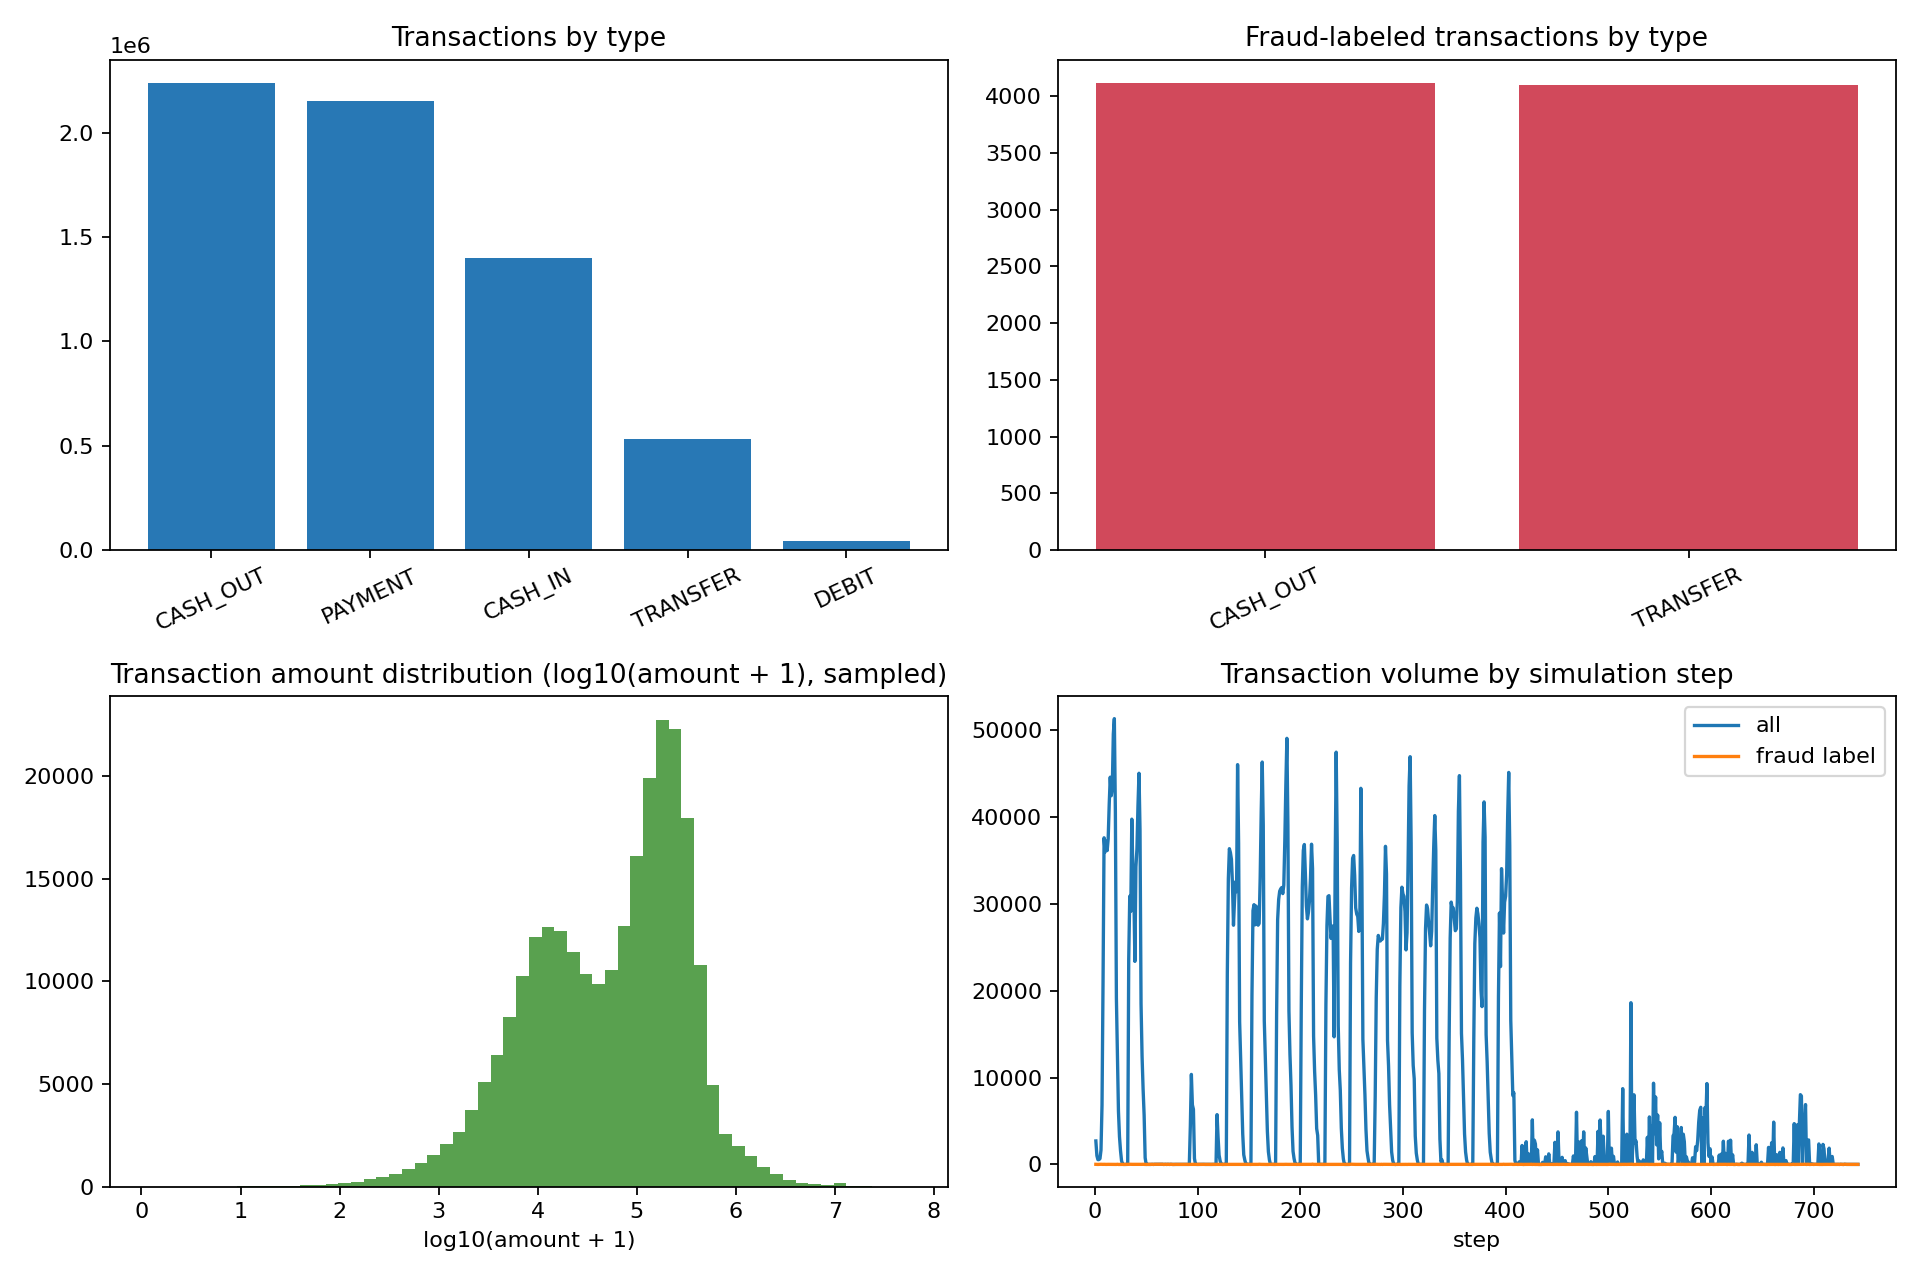
\includegraphics[width=.96\linewidth]{figures/eda_overview.png}\caption{Dataset overview. Amounts and account activity are sampled as described in the accompanying EDA summary.}\end{figure}
\section*{Feature construction and evaluation protocol}
The transaction task predicts the PaySim label $y_t\in\{0,1\}$. Account histories are derived only from strictly earlier simulation steps. Same-step transactions do not update one another because no within-step ordering is provided. Account IDs are used to join histories but are not classifier inputs; labels are excluded from aggregates.
\begin{table}[h]\centering\small\begin{tabularx}{\linewidth}{p{1.2in}p{2.6in}X}\toprule Feature set & Inputs & Purpose\\\midrule
A & Type, step, amount, pre-event source/destination balances & Transaction-only reference.\\
A without balances & Type, step, amount & Ablation for the simulator balance signature.\\
B & A plus prior endpoint counts, amount summaries, and time since last activity & Adds historical account behavior.\\
C & B plus prior distinct counterparties and repeat intensity & Tests simple graph neighborhood features.\\\bottomrule\end{tabularx}\caption{Feature sets and modeling purpose. Post-event balances, raw account IDs, and target-derived aggregates are excluded.}\end{table}
For a transaction at step $s$, behavioral snapshots contain events only through $s-1$. This avoids using the current transaction or assuming an order among events at the same step.
\begin{table}[h]\centering\small\begin{tabular}{lrrr}\toprule Split & Rows & Fraud rows & Fraud rate\\\midrule
Train ($s\leq520$) & 6,082,007 & 5,781 & 0.095\%\\
Validation ($521\leq s\leq631$) & 191,147 & 1,180 & 0.617\%\\
Test ($s\geq632$) & 89,466 & 1,252 & 1.399\%\\\bottomrule\end{tabular}\caption{Chronological evaluation split.}\end{table}
XGBoost uses histogram trees, learning rate 0.08, depth 6, minimum child weight 10, row and column subsampling 0.8, and L2 regularization 5. Training-only positive-class weight is 1,051.07. Validation AP controls early stopping (30 rounds; maximum 600 trees); the test set is reserved for final metrics. Logistic Regression uses class weighting. The rule baseline ranks transfer and cash-out transactions by log amount.
Average precision summarizes precision-recall ranking and is more informative than accuracy under severe imbalance. Operational results use exact alert budgets of 90, 448, and 895 test transactions; stable row order breaks tied scores.
\clearpage
\section*{Transaction classification}
Model A uses transaction type, amount, step, and pre-transaction balances; a separate ablation removes balances. B adds prior account behavior. C adds prior graph degree, distinct-counterparty, and repeat-intensity features. Models use a common chronological split. XGBoost uses histogram trees, training-derived class weighting, validation AP for early stopping, and a 600-tree cap. Alert metrics select exactly the top $k$ test rows with a stable tie-break.
\begin{table}[h]\centering\small\begin{tabular}{lrrr}\toprule Model & Validation AP & Test AP & P/R at 90 alerts\\\midrule
Logistic Regression & 0.386 & 0.517 & 1.000 / 0.072\\
XGBoost A & 0.951 & 0.971 & 1.000 / 0.072\\
XGBoost A, no balances & 0.249 & 0.326 & 1.000 / 0.072\\
XGBoost B, behavior & 0.911 & 0.938 & 1.000 / 0.072\\
XGBoost C, graph & 0.920 & 0.945 & 1.000 / 0.072\\\bottomrule\end{tabular}\caption{Transaction results. AP is average precision. At 90 alerts, recall is limited to 90 of 1,252 test frauds.}\end{table}
\begin{figure}[h]\centering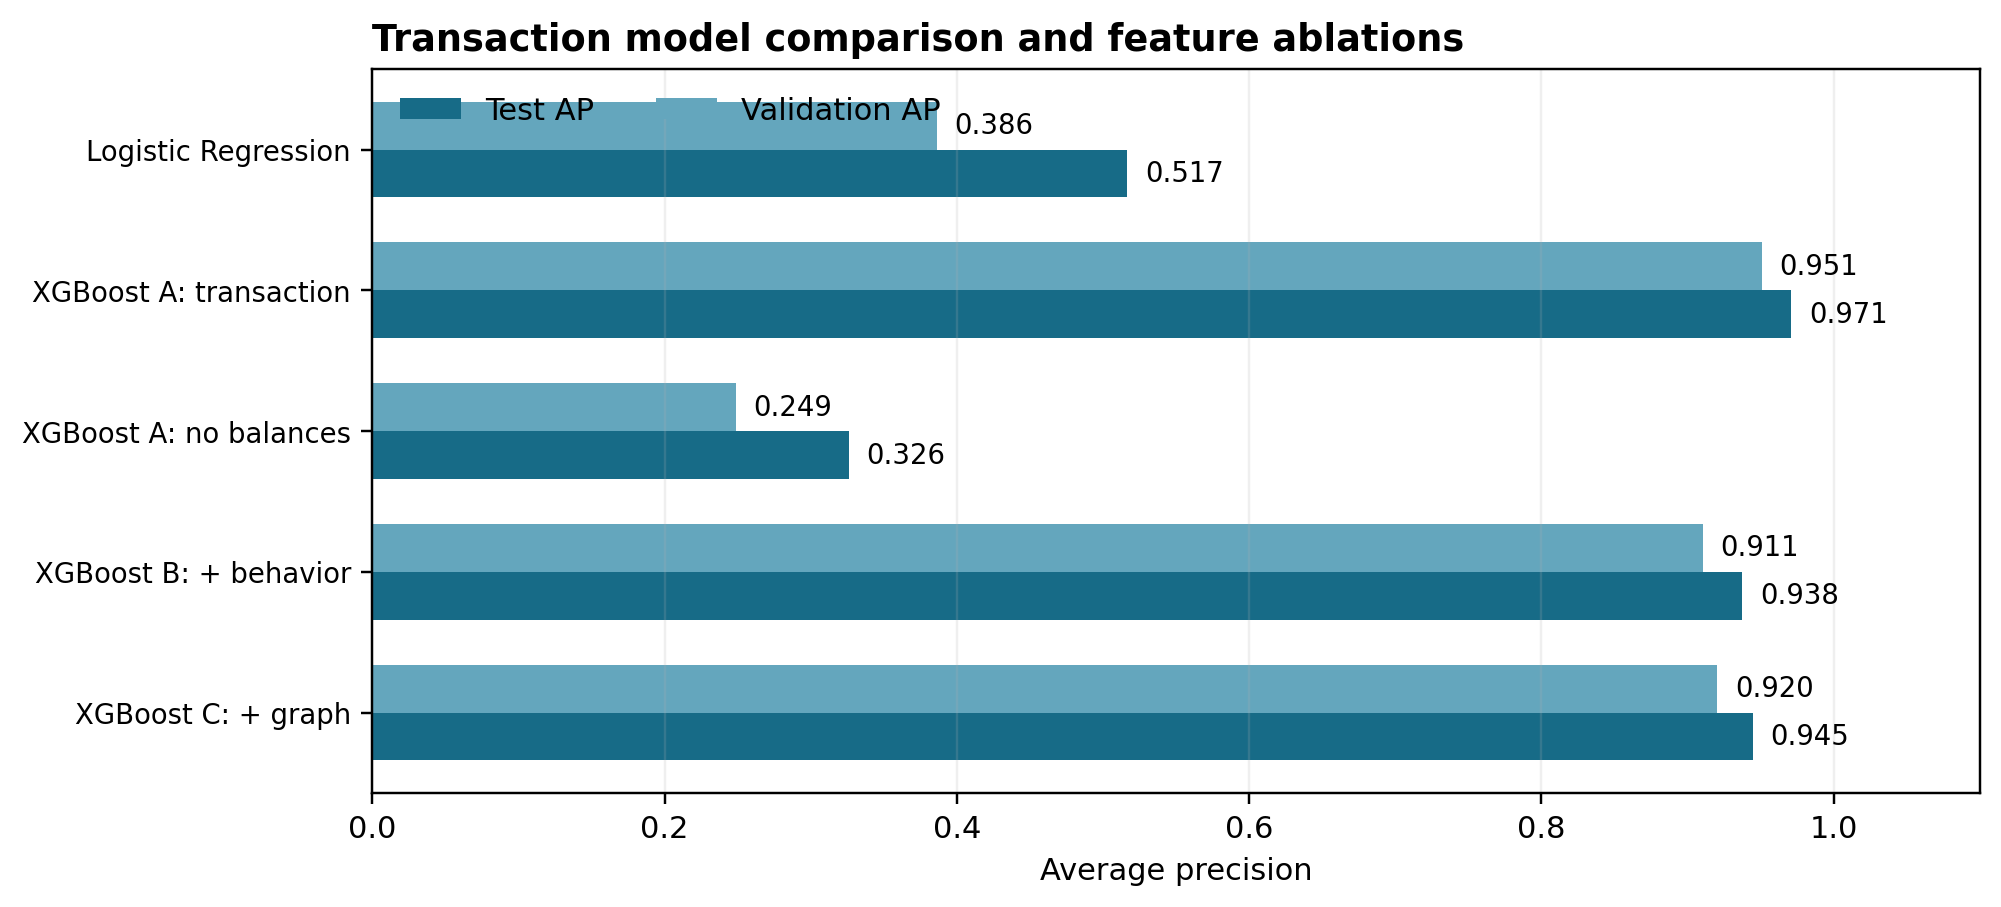
\includegraphics[width=.94\linewidth]{figures/classification_ablation.png}\caption{Validation and test AP by model and feature set.}\end{figure}
\textbf{Ablation finding.} 8,034/8,213 fraud rows (97.82\%) satisfy amount = oldbalanceOrg, compared with 0/6,354,407 non-fraud rows. These are pre-event fields, so this is not post-event leakage, but it is a simulator-specific shortcut. AP decreases from 0.971 (A) to 0.326 without balances. B reduces AP; C raises B by only 0.007 on test. A reaches the 600-tree cap and is not confirmed converged.
\clearpage
\section*{Operating points and interpretation}
\begin{table}[h]\centering\small\begin{tabular}{lrrr}\toprule Model & P/R at 90 & P/R at 448 & P/R at 895\\\midrule
XGBoost A & 1.000 / 0.072 & 1.000 / 0.358 & 0.990 / 0.708\\
A, no balances & 1.000 / 0.072 & 0.616 / 0.220 & 0.434 / 0.310\\
XGBoost B & 1.000 / 0.072 & 1.000 / 0.358 & 0.984 / 0.704\\
XGBoost C & 1.000 / 0.072 & 1.000 / 0.358 & 0.989 / 0.707\\\bottomrule\end{tabular}\caption{Precision and recall at exact test alert counts.}\end{table}
\begin{figure}[h]\centering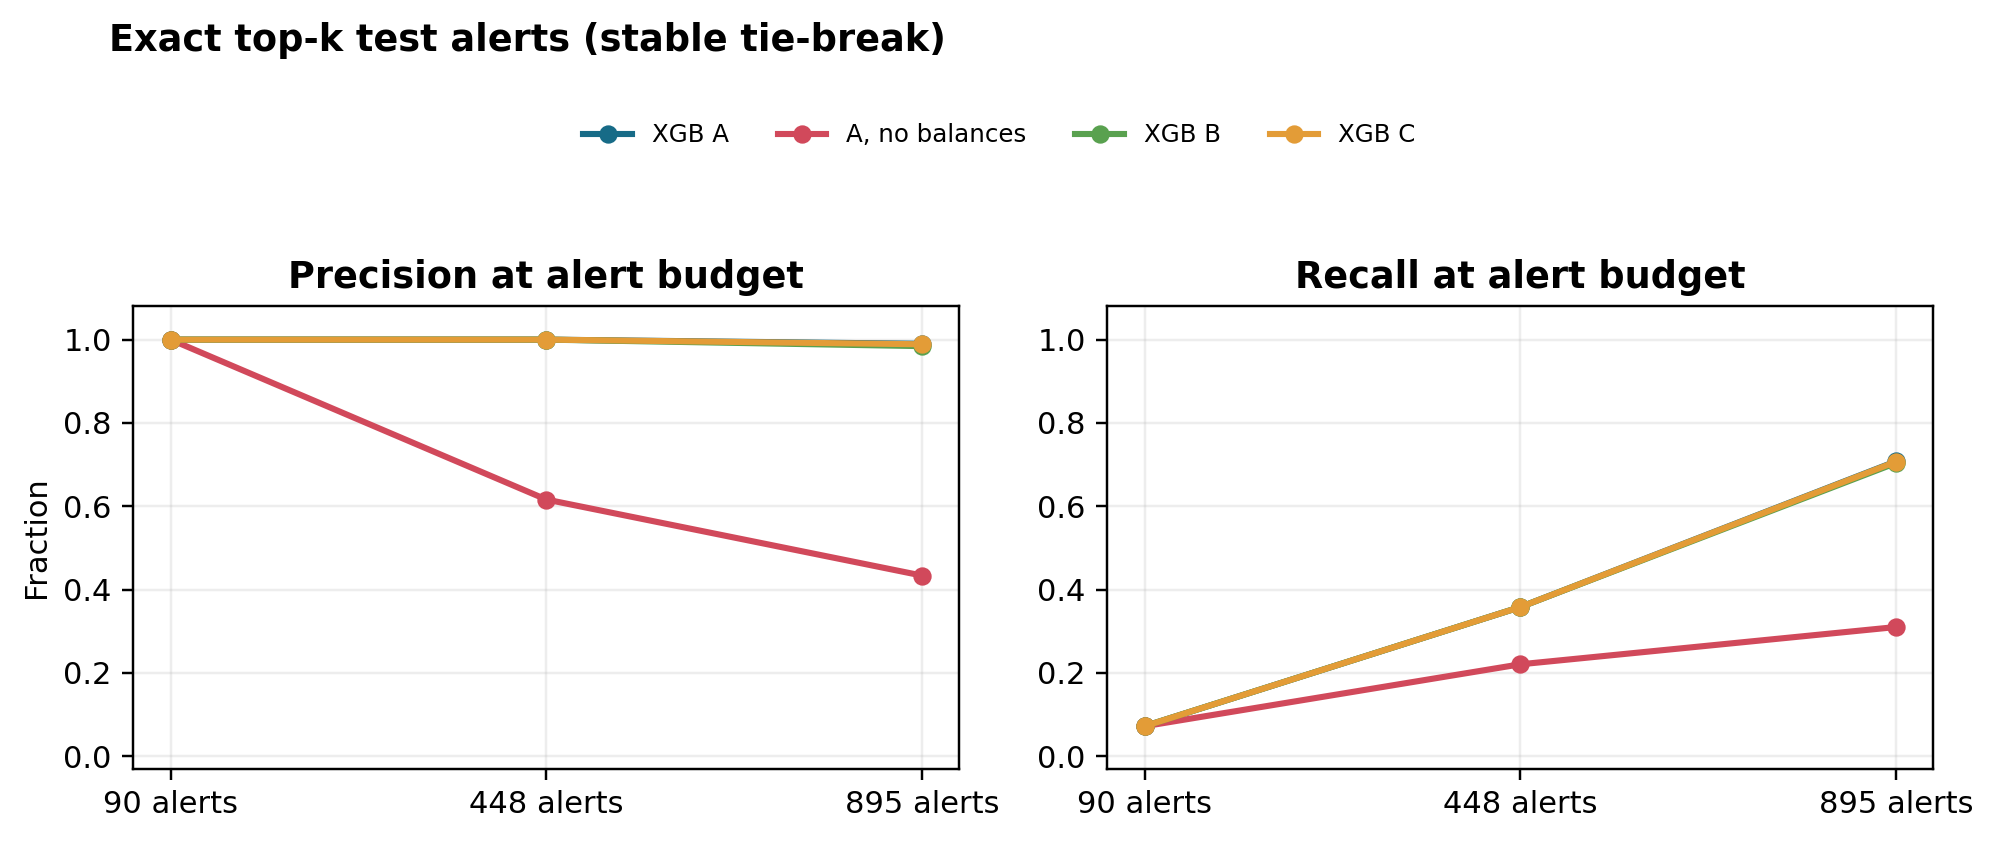
\includegraphics[width=.94\linewidth]{figures/alert_budget_results.png}\caption{Precision and recall under exact test alert budgets for XGBoost variants.}\end{figure}
At 90 alerts, each XGBoost variant retrieves the same 90 frauds and no false positives, so recall is only 7.19\%. At 448 alerts, A, B, and C each recover 448 frauds; the balance-free model recovers 276. At 895 alerts, A, B, and C remain close. Graph features improve B by only 0.0074 test AP and do not surpass transaction-only A.

At the 90-alert score cutoff, a threshold-inclusive rule would select 93 A rows, 214 no-balance rows, 199 B rows, and 165 C rows. Metrics instead use an explicit stable top-$k$ tie-break to honor the review capacity. A real deployment would need an explicit secondary ranking or queue rule for tied scores.
\clearpage
\section*{Candidate-group discovery}
The separate group miner does not read fraud labels or classifier scores. It uses non-overlapping 24-step windows and proposes weak components, strongly connected components, fan-in/fan-out motifs, and Charikar-style dense subsets. A candidate must contain at least three accounts in a directed cycle or two temporally ordered relay accounts across multiple active steps. A fixed evidence score combines structure, transaction timing, repeated pairs, amount similarity, and flow continuity; it is a ranking heuristic, not a probability.

The complete scan covered all 31 windows and returned zero eligible PaySim groups. This means none passed the chosen screen, not that fraud rings are absent. Without verified ring IDs, PaySim ring precision/recall cannot be calculated. On a controlled benchmark of 30 planted groups and 90 decoy episodes per seed (five seeds), the group score obtained mean AP 0.241 (SD 0.040), precision@30 0.447 (0.069), member recovery@30 0.357 (0.055), and ring recall@30 0.447 (0.069). Matching uses one-to-one account-set IoU >= 0.5. This synthetic benchmark does not validate real-world performance.
\begin{table}[h]\centering\small\begin{tabularx}{\linewidth}{p{1.35in}X}\toprule Stage & Evidence and decision\\\midrule
Proposal & Weak components bound membership; SCCs, fan-in/fan-out, and dense peeling add overlapping subgraph proposals.\\
Coordination evidence & Ordered inflow then outflow, activity span, repeated pairs, flow continuity, and amount similarity.\\
Eligibility & At least three accounts in a directed cycle, or two temporally ordered relays across multiple active steps.\\
Ranking & Fixed weighted heuristic for review priority; not a calibrated probability and not trained on PaySim labels.\\\bottomrule\end{tabularx}\caption{Candidate group proposal, eligibility, and ranking are separate stages.}\end{table}
Strict criteria may miss longer or cross-window groups, weakly connected rings, and partially observed behavior. Windows are non-overlapping; dense-subgraph peeling is limited to components of at most 20 accounts. These bounds limit computational work but create false-negative risks.
\section*{Conclusions and limits}
The strongest transaction result is inseparable from a synthetic balance signature; balance-free AP is materially lower. Behavioral and graph features do not outperform transaction-only XGBoost on AP. The group workflow is a candidate miner, not a validated fraud-ring classifier, and this run yielded no eligible PaySim groups. The controlled experiment gives a reproducible but modest ring-recovery check. Additional time cutoffs, noisy/overlapping planted groups, larger-scale sensitivity checks, and independently labeled real data are needed before making generalization claims. Streaming remains future work.

\textbf{Reproducibility.} Commands are in README.md. Metrics, saved test predictions, data profile, EDA, full group scan, and five-seed benchmark are in outputs/.
\end{document}
